% XeLaTeX can use any Mac OS X font. See the setromanfont command below.
% Input to XeLaTeX is full Unicode, so Unicode characters can be typed directly into the source.

% The next lines tell TeXShop to typeset with xelatex, and to open and save the source with Unicode encoding.

%!TEX program = xelatex
%!TEX TS-program = xelatexmk
%!TEX encoding = UTF-8 Unicode

\documentclass[authoryearcitations]{UoYCSproject}
\author{Andrew Durant}
\title{Developing a platform for common evaluation of self-healing in wireless sensor networks}
%\date{}
\supervisor{James Harbin}
\CSESE
\wordcount{0}

\includes{}

\excludes{}

\abstract{Wireless sensor networks are used in a wide range of applications, and in recent times this is only expanding. Due to them being small, low-power devices, and the common network connectivity using multi-hop routing: network drop-outs and partitioning of devices is a common problem. According to \citet{Tong2009} self-healing by means of mobile nodes still remains a greatly unstudied area. However, more recently developments have been made in diverse ways.

There are two main approaches to network and device management for combating and fixing these issues, the distributed approach and the centralised approach. However the application for a particular WSN determines the effectiveness of a particular algorithm or management paradigm. In certain use cases power usage is less likely to be an important contributing factor but speed of detection and recovery will be more pressing. Whereas in an environmental monitoring situation network nodes are more likely to be physically difficult to get to once deployed, and longevity of battery power is highly important.

With these considerations, performance metrics given for particular algorithms may not give a fair comparison, as algorithms optimised for low power consumption have a very different purpose to those optimised for rapid recovery. Because of this a common platform for comparison between approaches to self-healing is desired.}

\dedication{}

\acknowledgements{}

% More definitions & declarations in project-report.ldf

\makeatletter
\def\ext@algorithm{lol}% algorithm captions will be written to the .lol file
% share the list making commands and redefine the heading
\AtBeginDocument{%
  \let\l@algorithm\l@lstlisting
  \let\c@algorithm\c@lstlisting
  \let\thealgorithm\thelstlisting%
}
\makeatother
\makeatletter
\newlength{\singlespace}
\newlength{\gobble}
\newlength{\numbersep}
% The width of a single space.
\settowidth{\singlespace}{\lst@basicstyle \ }
\setlength{\singlespace}{-\singlespace}

\lst@Key{firstlineandnumber}\relax{\def\lst@firstline{#1\relax}\def\lst@firstnumber{#1\relax}}
\lst@Key{widthgobble}{0}{%
    \setlength{\gobble}{0.9\singlespace}% reindent a bit
    \setlength{\gobble}{\lst@tabsize\gobble}% multiply by tabsize
    \setlength{\gobble}{#1\gobble}% multiply by number of tabs
    \def\lst@xleftmargin{\gobble}% move left margin left
    \def\lst@framexleftmargin{\gobble}% move left frameborder left
    \setlength{\numbersep}{\gobble}%
    \addtolength{\numbersep}{10pt}%
    \def\lst@numbersep{\numbersep}% distance between numbers and left frameborder
}
\makeatother

\begin{document}
\maketitle
\listoffigures
\listoftables
\renewcommand{\lstlistlistingname}{List of Listings}
\lstlistoflistings

\chapter{Introduction}
\label{cha:Introduction}

\section{Project Aims}

This project aims to investigate self-healing in wireless sensor networks. Research will investigate the current developments in this field leading to a need for a common evaluation tool for approaches to self-healing.

The goal of this project is to produce a wireless sensor network simulation platform as a reference architecture for evaluating self-healing algorithms. The applications of this range from academic investigation during the development of new algorithms or the improvement of existing algorithms, to practical evaluation of candidate systems prior to development and deployment. The platform will be able to simulate and visualise any algorithm implementation on a realistic network.

The project does not aim to produce a novel self-healing algorithm, but during evaluation will suggest what features are critical for general and specific applications, and areas in which it would be useful to focus future research and algorithm development.

\section{Report Structure}

The body of this report consists of 5 chapters that each describe the tasks within the project.

In chapter~\ref{cha:LitReview} the existing literature and work in self-healing wireless sensor networks is reviewed to gain an in-depth understanding of the current state of research, the problems being solved, and how those solutions are evaluated. Each of these topics are categorised in their own section.

Analysis of the problem and the scope of the project is described in chapter~\ref{cha:Problem}, this chapter sets out the objectives that this project is aimed to achieve.

The design and implementation of the project is detailed in chapter~\ref{cha:Design}, describing the decisions made and the reasoning for them, and the specifics of how the system has been built.

Chapter~\ref{cha:Eval} evaluates the systems produced in chapter~\ref{cha:Design} against the metrics discussed from chapter~\ref{cha:LitReview}. The chapter also evaluates the platform itself.

The report is concluded in chapter~\ref{cha:Conclusion} with a review of the results produced and the conclusions that can be made from them. The chapter returns to the objectives defined in chapter~\ref{cha:Problem} and reviews their status. The report is then finished with suggestions for future work in this area, and further development of the platform.

\section{Statement of Ethics}

The intended application of this project is academic. However, there are potential applications for the methods and algorithms discussed for monitoring or affecting humans, animals or the environment. This project does not include such examples and carries no malicious intent.

The project does not involved any human participants. No sensitive information, that could have a negative impact on any person or organisation, has been gathered during the project.

\chapter{Literature Review}
\label{cha:LitReview}

% Introduction

In order to consider self-healing in real-world applications of wireless sensor networks an understanding of the possible applications is required. A survey of approaches to self-healing is then presented along with metrics that can be used to evaluate and compare them. This is followed with a review of evaluation techniques and real-world factors for wireless sensor networks.

\section{WSN applications}

% JAMES %
% Condense the description in 2.1 and potentially move some of this text
% into the general introduction, if you need the word count

The possible applications for wireless sensor networks are diverse and far reaching. The small self-powered devices that can gather data from a wide area, to detect events and communicate information back to a base station either processed or for processing lend themselves to a large number of applications. Each of these applications utilise the WSN in different ways and thereby bring new challenges to the developer of the systems. Due to this the design of the network is highly dependent on the application domain. Just some of the fields WSNs have been used in are environmental monitoring, warfare, agriculture, surveillance, medical care, education and micro-surgery.

Habitat monitoring using WSNs has been taking place on an island of ducks where ordinary monitoring techniques cause disturbance to the animals with problems such as increasing mortality and eventual abandonment of the habitat. The use of WSNs that can be deployed prior to seasonal habitation enables constant monitoring over the time without the need to disturb the inhabitants. \citet{Mainwaring2002} detail the requirements of the network and how it has been developed. Longevity of the devices, remote management, and inconspicuous operation are required to ensure the WSN is reliable and the data is able to be collected. The locations used for WSNs are often extreme, particularly for habitat monitoring. Similar requirements to the above are generated by \citet{Biagioni2002} for monitoring endangered plants. Most importantly however for collecting scientific data is ensuring the system is reliable and the user can have confidence in the data.

% JAMES %
% "ensuring the system is reliable" - what measures did they
% take to do this, and what potential failures were assumed? This can
% give insight into the types of failures real applications expect

A very different approach was taken by \citet{Juang2002} in developing ZebraNet. Rather than statically positioned nodes, the devices are attached to the herd of zebra being monitored with collars. The nature of this system is entirely mobile, without even a fixed base station to report to. Because of this the nodes pass data between them when within range forming a distributed collection and storage network. The mobile base station can then be deployed occasionally to collect the dataset only needing to meet a few devices to obtain all of the data gathered by the network. This network is inherently ad-hoc where nodes may or may not come into contact with one another frequently, and there is no fixed or permanent base station to report to. Again longevity is an important requirement as deploying or re-deploying the sensors requires capture of the animals, so the systems must run for at least a year with no intervention.

Environmental monitoring on volcanoes has been investigated by \citet{Werner-Allen2006} where the use of WSNs enables data collection over a wider area for a longer amount of time compared to using traditional equipment. WSN nodes can be deployed easily and left unattended to monitor the volcano area over a period of several weeks or months. Whereas traditional equipment is bulky and heavy, and therefore difficult to deploy limiting the area of research. The WSN transmitting the collected data back to the base station also removes the need to frequently return to the sensor devices to retrieve data. This is a clear example of using the advantages of wireless sensor networks. However a number of potential issues are raised. The nodes are deployed at the limits of their range to the nearest neighbour, this allows as large an area as possible to be covered, however if a single node fails all other nodes that were dependent upon it will be unreachable. In the scale of this network, where the maximum hop length from the base station is 6 this may seem insignificant, however that is 37.5\% of the network nodes.


\section{Approaches to self-healing in WSNs}



\subsection{Centralised}

The main way centralised approaches are used in WSNs is in the configuration of the network structure to minimise energy use and ensure good coverage of the area of interest \citep{Wang2003,Ding2005,Wang2005,Derr2013}. Centralised evaluation of the network and area of interest prior to deployment ensures the connectivity and coverage requirements of the application are met.
\begin{quote}
Coverage requires that every location in the sensing field is monitored by at least one sensor. Connectivity requires that the network is not partitioned in terms of nodes' communication capability. Note that coverage is affected by sensors' sensitivity, while connectivity is influenced by sensors' communication ranges.
\citep{Wang2005}
\end{quote}
These vary by application for instance, detection and localisation of events require multiple nodes covering smaller areas (a dense coverage) whereas other applications may only need one node within its transmission range (a sparse coverage). By pre-planning to match the deployment to the application needs the network will be much more efficient in power use and accurate in data collection.

Networks with a high degree of connectivity are more resilient to node failures. \Citet{Wang2003} investigate the relationship between coverage and connectivity to produce an integrated solution that is able to maintain both requirements whilst reducing energy consumption. The degree of connectivity is described as $K$-connected, where any $K-1$ nodes may fail without loosing network connectivity. So the higher the connectivity ($>K$) the more nodes are able to fail without disrupting the rest of the functioning network.

% JAMES
% 2.2.1 - but does pre-planning risk placing nodes too thinly in the
% event of failure? Trade off could be commented upon
%
% done

Connectivity is important as simply achieving area coverage would result in nodes being placed too thinly in the event of failures, either requiring a large movement in the network or simply not being able to recover. The main goal of pre-planned centralised approaches is to create a deployment that is resilient without further intervention.

Due to the differences in applications a number of application specific methods have been proposed in addition to those previously mentioned \citep{Meguerdichian2001,Meguerdichian2001a,Meguerdichian2003}. All of these provide for different application requirements in different ways. However a single parametrised method that can be applied to many differing applications has been developed by \citet*{Derr2013}. This allows the specification of the number of nodes and the distance between the nodes which defines the desired coverage and connectivity respectively. The algorithm first constructs a triangle based mesh for the given area of interest, for example with NETGEN (Figure~\ref{fig:netgen}), however this creates more nodes than desired. To reduce the number of nodes \citeauthor*{Derr2013} create the mesh simplification algorithm INRCDTS which removes nodes and smooths the mesh until the required number of nodes from the desired network parameters is reached (Figure~\ref{fig:inrcdts}). To ensure that both coverage and connectivity requirements are met the algorithm assumes that the communication range ($R_C$) is greater than $\sqrt{3}$ of the sensing range ($R_S$) i.e.\ $R_C \ge \sqrt{3} R_S$. Based upon this assumption the nodes spacing is determined by $\sqrt{3} R_S$ which ensures coverage and therefore connectivity for the network.

\begin{figure}
 \centering
    \begin{subfigure}[t]{.48\textwidth}
        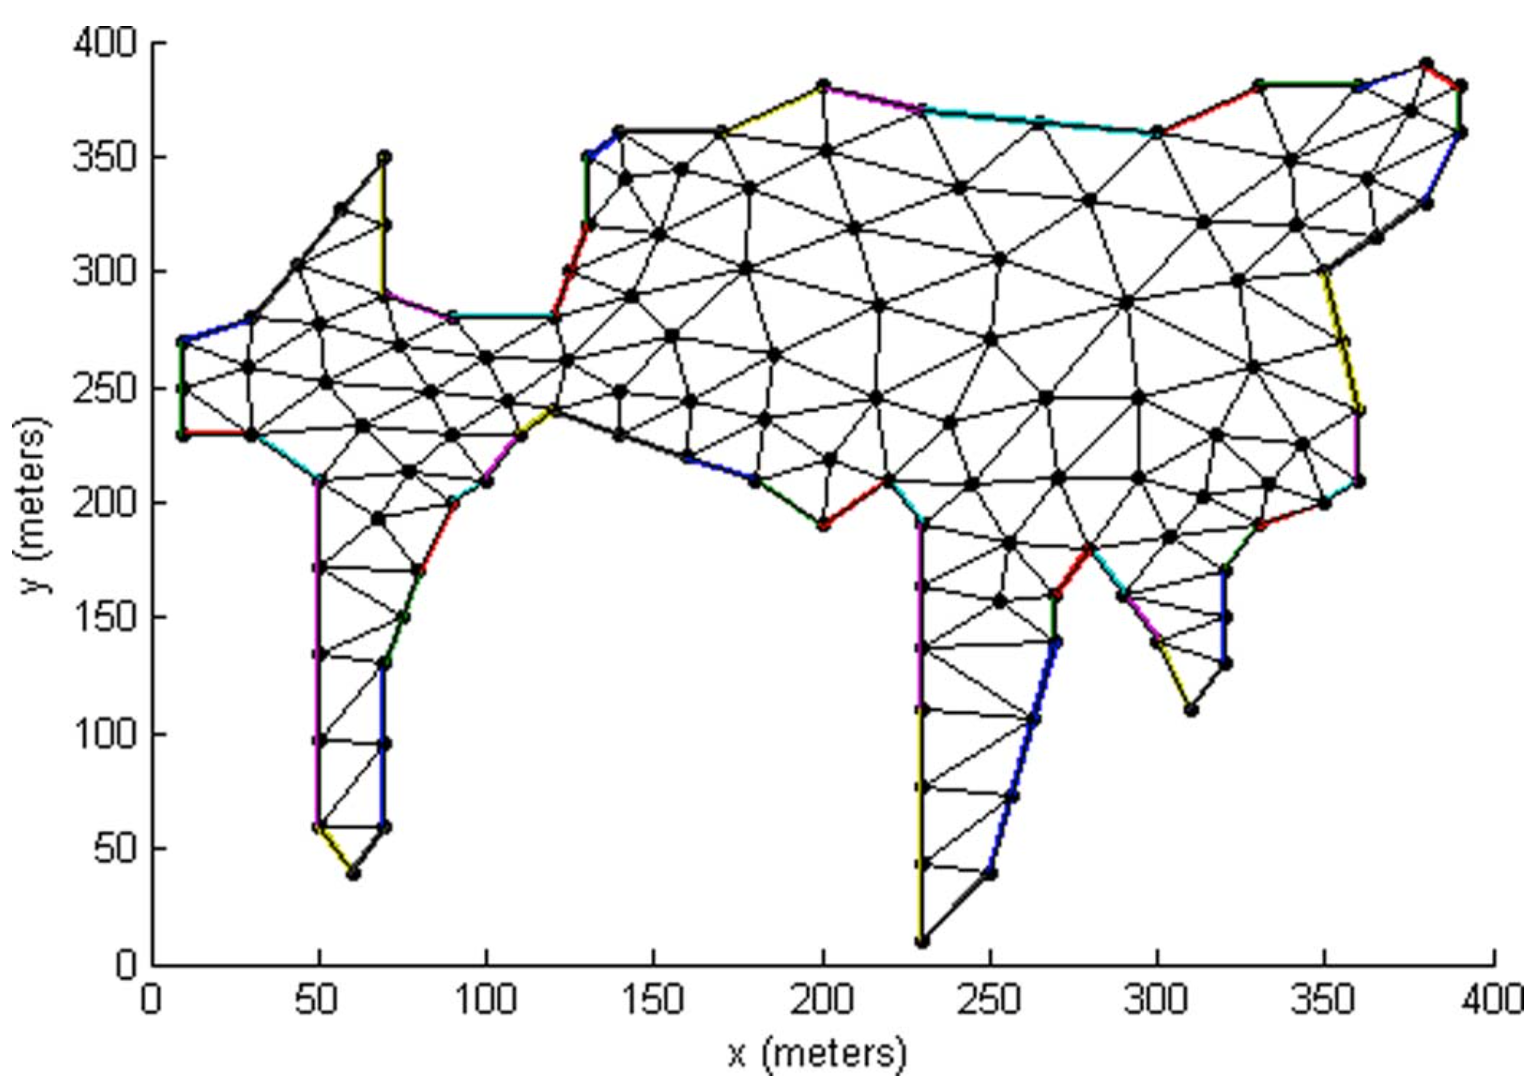
\includegraphics[width=\textwidth]{figures/netgen.png}
        \caption{Mesh generation with NETGEN, maximum edge length of 40; 126 nodes.}
        \label{fig:netgen}
    \end{subfigure}
    ~
    \begin{subfigure}[t]{.48\textwidth}
        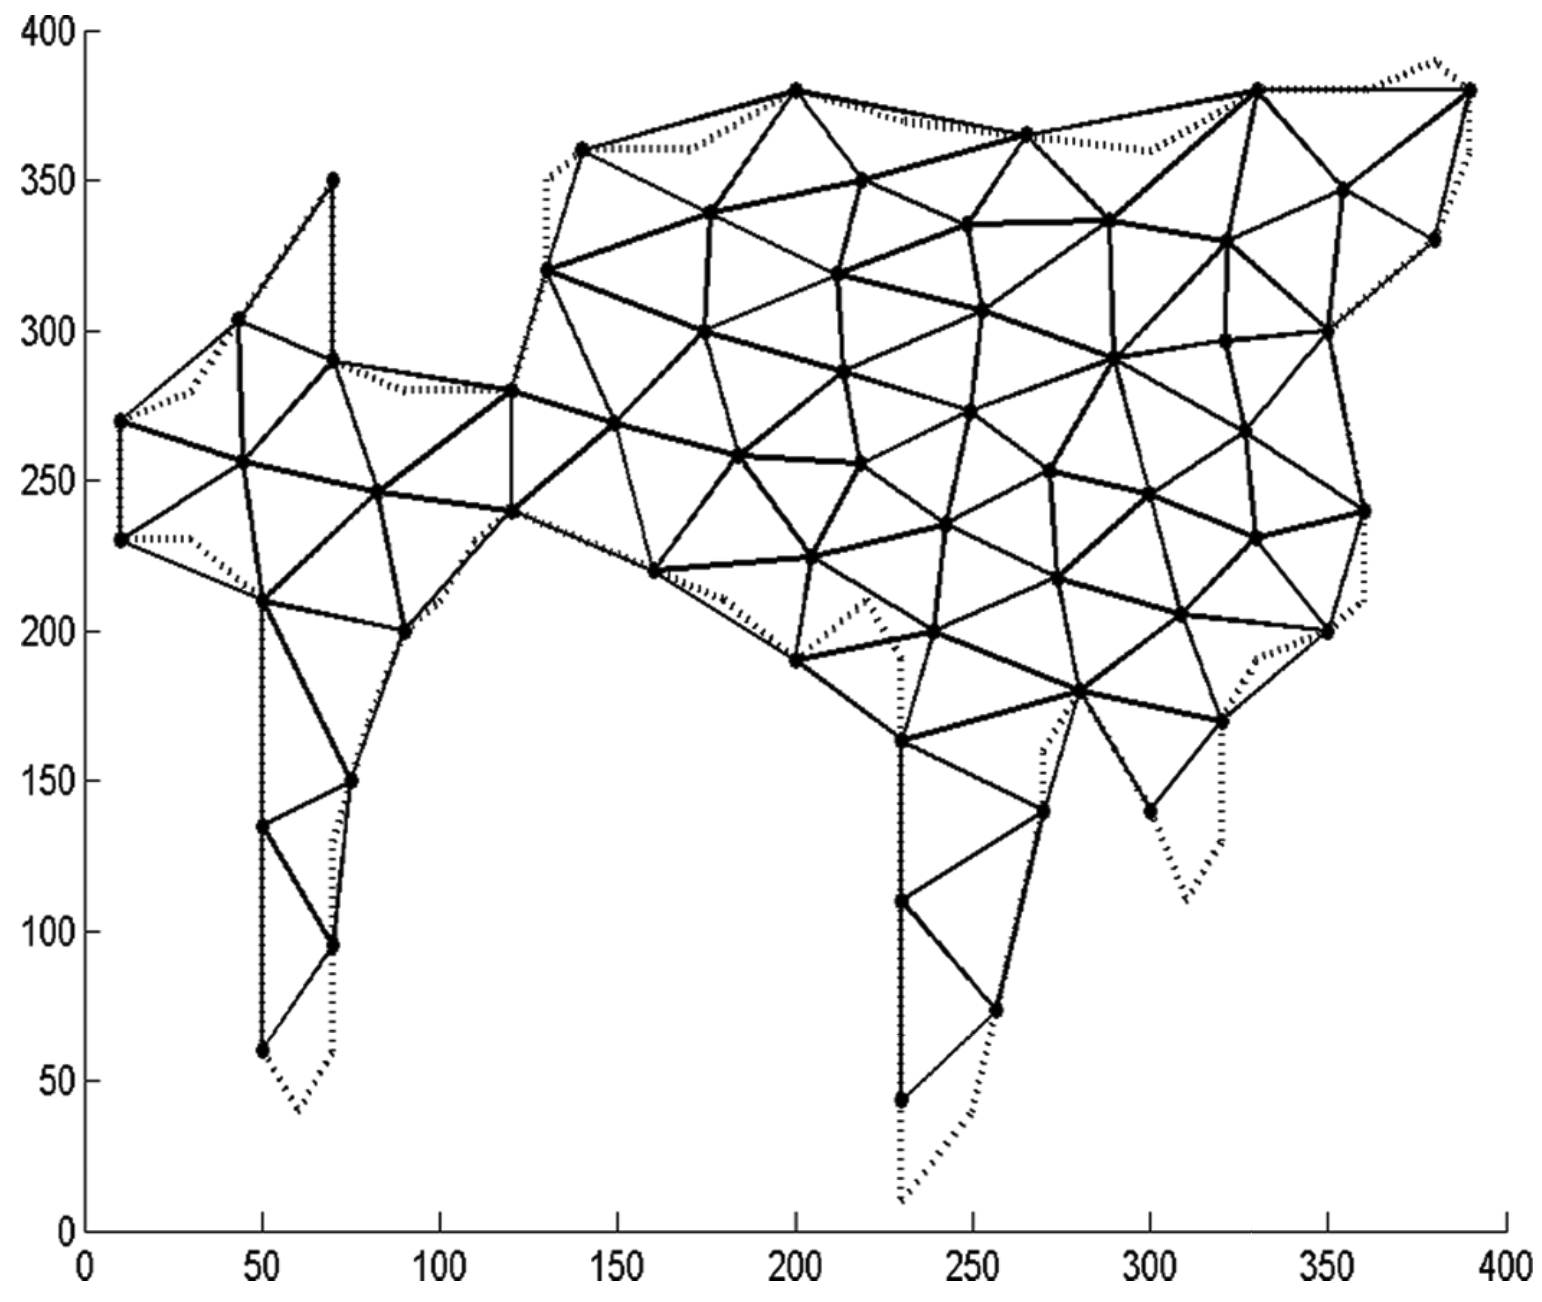
\includegraphics[width=\textwidth]{figures/netgen-inrcdts.png}
        \caption{NETGEN mesh simplification with INRCDTS algorithm; 60 nodes.}
        \label{fig:inrcdts}
    \end{subfigure}
 \caption{Mesh generation and simplification.}
 \label{fig:netgen-inrcdts}
\end{figure}

% JAMES
% More detail on citation [8], the parametrised method of Derr and
% Manic, as we discussed last time.
%
% done

Most centralised approaches use a priori information to specify exact deployment in the area of interest. However \citet*{Qu2012} have developed a post deployment particle swarm optimization (PSO) algorithm that is computed centrally to provide optimal coverage and reduce energy consumption. A centralised algorithm is able to understand the entire network, available devices, and area, and therefore produce the optimal distribution of nodes. The nodes are on a mobile platform that is able to move within the area. Reduction of energy consumption is done by dynamically reducing the range of sensing and communication on each device to the minimum needed once the locations have been determined. \citeauthor*{Qu2012} do not address node failures, as they assume all node are working throughout the time of use. The distance measurement is also assumed to be for a point-to-point movement with no consideration for difficulties navigating the terrain. The energy considerations take account of the mobility and sensing of the node, the other components power usage is ignored as it is not increased by the algorithm. The centralised calculations for deployment take place on a device with unlimited power. The significance of the algorithm is dependent upon the relative energy consumption of sensing and movement. If sensing requires more energy then the algorithm can provide significant improvements, however when movement has a higher energy cost the saving is negligible.

No consideration is made for the energy cost of transmitting additional messages back to the root node, this is a concern as if all messages must be relayed back, the nodes near the top of the tree will have a significantly larger number of messages to receive and transmit, reducing their lifetime dramatically. This is partly mitigated by the algorithm only running at deployment rather than throughout, however the nodes closest to the root will still be depleted first, and therefore cut off communication in the network. Provision should be made for this, but \citeauthor*{Qu2012} leave it unmentioned.

% JAMES
% Qu and Georgakopolous... is their energy reduction taking into
% account the additional costs of coordinating via the sink
% nodes?
%
% done
%
% concerns over missing information

\subsection{Distributed}

In \citet{Abbasi2007}'s seminal paper DARA (a Distributed Actor Recovery Algorithm) is introduced. Developing a localised scheme to restore a network of mobile nodes when it has become partitioned due to a node failure. The distributed nature of the algorithm avoids involving every single node, only requiring the local nodes to respond. The algorithm selects a node to replace a failed node and coordinates the local nodes to relocate to rebuild the network. As nodes relocate they may cause other partitioning, but this is dealt with in the same way forming a chain reaction until the entire network is reconnected. The self-healing process requires no supervision or centralised control. The use of cascaded movement reduces the overall movement of nodes as instead of entire blocks moving to recover only a few nodes are needed. This contributes to the main goal of minimising the total distance moved by the network nodes.
DARA produces particularly bad results when used with cyclic network topologies. When the node movement is cascaded the entire cycle of node will be moved, when only one may need to be for the optimal solution. To combat this a variant that sends flooding messages to check connectivity before moving is produced. This increases message overhead, but can significantly reduce node movement which tends to be more power hungry.

PADRA \citep{Akkaya2008} also aims to restore connectivity to a local area after a node has failed, whilst minimising the total distance travelled, and without external supervision or involvement. However unlike DARA it provides the functionality to detect the cut-vertices that are the cause of partitioning. PADRA determines potential cut vertices in advance by forming a connected dominating set of the whole network. The dominating set is also used for selection of recovery nodes as the dominating node moves to recover the network. Through this PADRA improves significantly upon DARA towards total travel distance of the optimal cascade model.

RIM (Recovery through Inward Motion) \citep{Younis2010} improves upon DARA and PADRA which each need 2-hop knowledge of the network to only requiring 1-hop knowledge on each node. This significantly reduces the network overhead for maintaining the required knowledge of the network topology, however the simplicity means that the distance travelled by the nodes is greater in larger networks for RIM than for DARA or PADRA. Calculating and transmitting a lot of detailed information is often considered too much overhead for low-power, low-complexity systems, particularly if the network can change often or easily. Depending on the application for the WSN the communication overhead to maintain the topology data could be justified over the generally more efficient algorithm.

Another flaw in RIM is that it assumes and requires only one node failure at a time. Whilst this may be the case, failures in WSNs are most commonly battery depletion, which is likely to occur at similar times across the network, or random failure due to environmental conditions, which could happen at any time to one or multiple nodes.

\begin{figure}
 \centering
    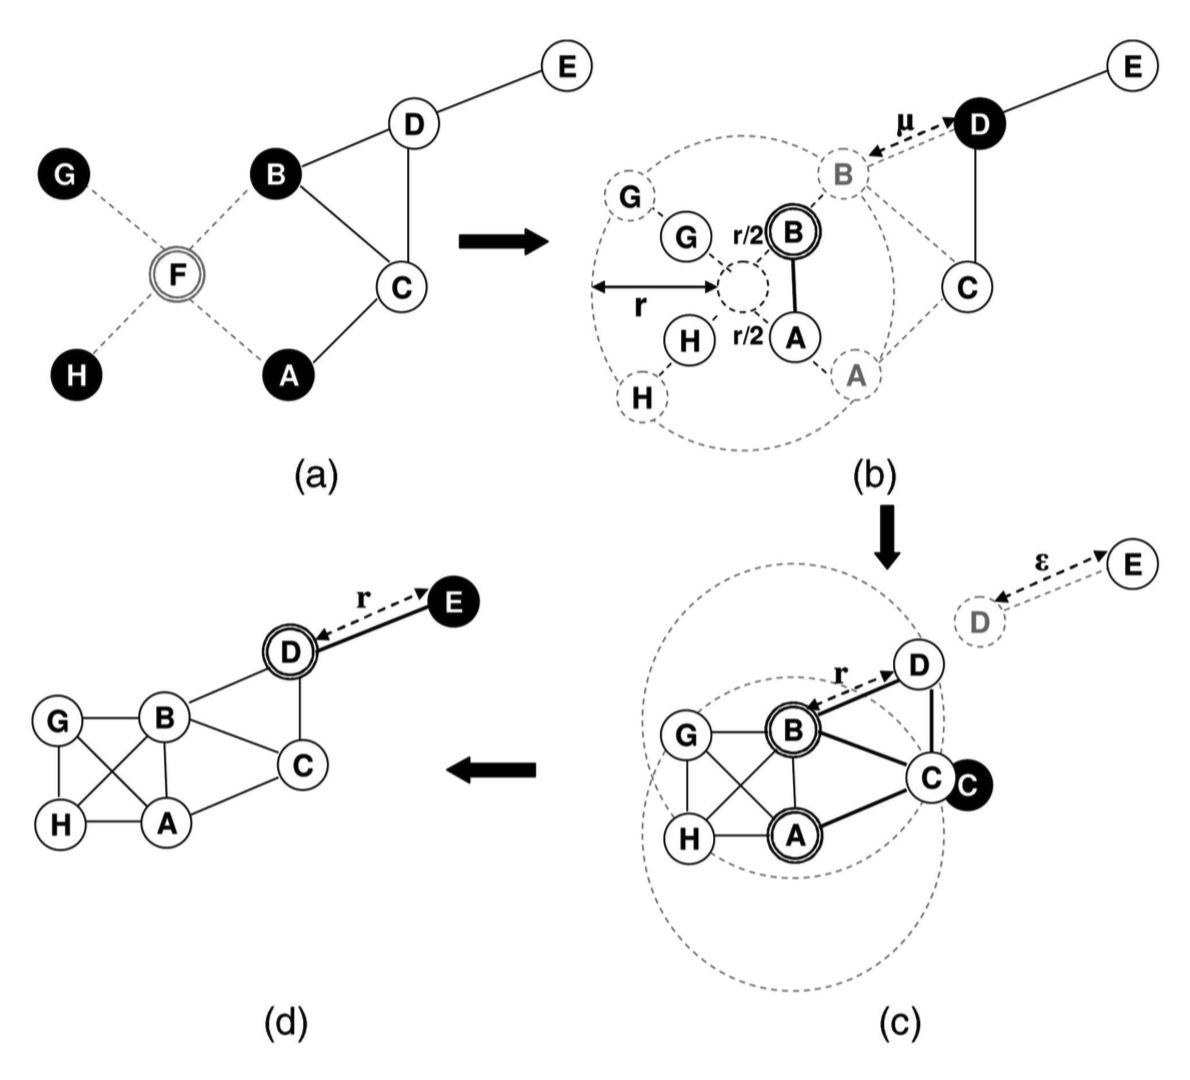
\includegraphics[width=0.6\textwidth]{figures/rim.png}
    \caption{(a)--(d) An example for how RIM restoration process; each shaded node moves based on the position of its neighbours, denoted in double-lined circles.}
    \label{fig:rim}
\end{figure}

% JAMES
% DARA, PADRA and RIM... what results do they give and how were they
% evaluated in their papers.

% a bit more explanation of diagrams / annotations

SFRA \citep{Alfadhly2012} is designed specifically to deal with multiple simultaneous failures to combat the multiple failure problem in RIM. Network trees are built from the root node, with local cluster-head nodes, this introduces a fair amount of network overhead compared with RIM. The number of updates needed to send is reduced by waiting for all child node messages before propagating back up the tree.

\begin{figure}
 \centering
    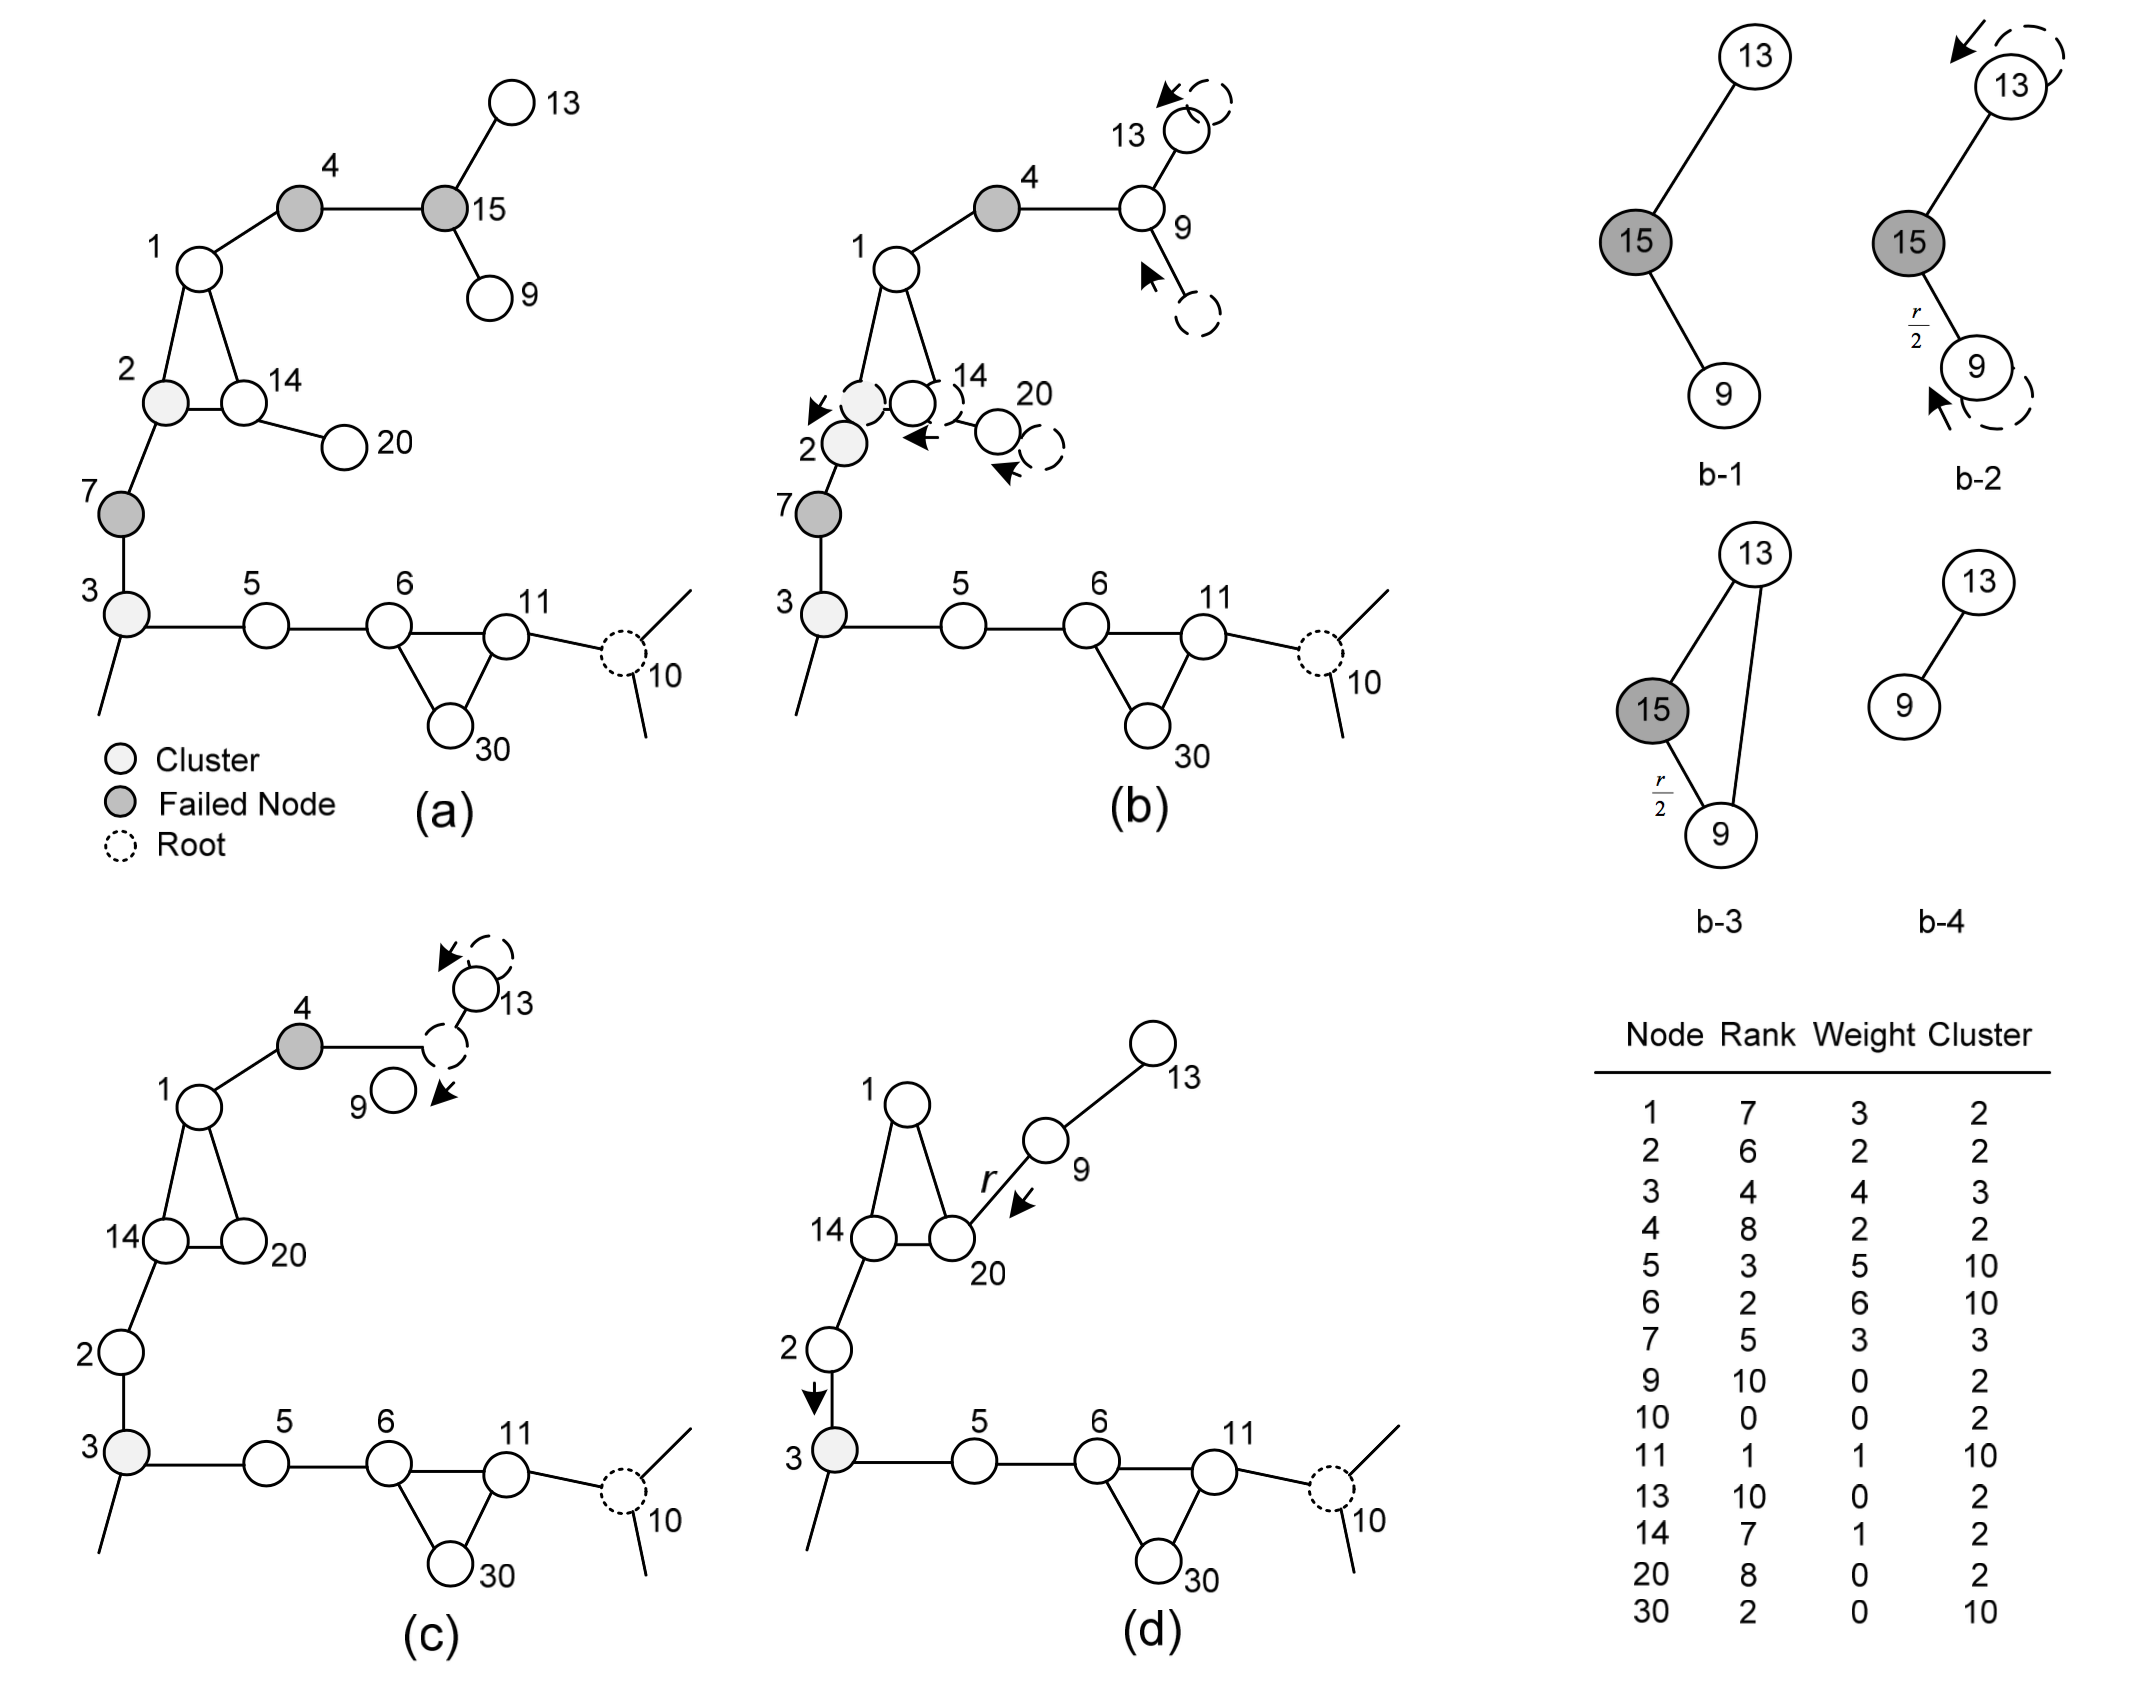
\includegraphics[width=\textwidth]{figures/sfra.png}
    \caption{Detailed example to illustrate how SFRA algorithm restores connectivity after multiple nodes fail.}
    \label{fig:sfra}
\end{figure}

Distributed approaches become much more efficient as the network scales because they are only concerned with the local nodes that are directly reachable. This allows networks built upon distributed algorithms to become much larger, and cover much wider areas as the overhead increase from additional nodes is minimal compared with the exponential increase in complexity from the centralised approaches.

A number of biologically-inspired approaches exist utilising animal and insect coordination and inspired methods of load balancing. \citet{Caliskanelli2014} suggests the application of bee pheromone based load balancing to node distribution. The main thesis applies pheromone signalling (PS) to node redundancy enabling and disabling nodes within a dense area to preserve their life when they are unneeded. By deciding upon a cluster head for an area all other nodes move to a dormant state but coverage is maintained. If an active cluster head fails then a new cluster head will be assigned. Each cluster head emits a pheromone signal that prevents other nodes from becoming the head. PS is then applied to robotic agents to increase service availability though guidance to specific locations. A pheromone signal denotes coverage of a particular area, in load balancing if an area does not have a strong enough signal an node will be activated to provide coverage and emit pheromone to show it. For robot guidance the agents move towards areas that are lacking in pheromone signal as these will be areas in which nodes have depleted their battery or failed.

% JAMES
% pg 12. Ipek's thesis on node distribution... you have phrased it in
% the form of "each node could". I think there is an exact definition of
% in a later chapter of how the mobile robots operated.
%
% done

Another approach based upon the behaviour of ants in a colony has been introduced by \citet{Wang2014}. The system separates mobile nodes from the normal sensor nodes that are static. The network functions as normal on the static nodes. However if there is a need for relocation of a node, due to failure or any other cause, the mobile nodes can pick up the static nodes and travel with them to another location redeploying them there. This reduces the power and cost overheads of adding mobility to all of the nodes. The mobile nodes can carry a larger battery or travel to a charging station when not actively moving nodes.

% JAMES
% How do the bio-inspired protocols contrast critically with each other?
% Comment on notable differences in performance achieved in the papers,
% realism of any dependencies, and the types of failures protected
% against.

% difference in message overhead, control message transmission etc. - assumptions made - failure modes able to recover - time to recover - topologies tested with, random structured etc. - hardware, simulation

A similar approach has been taken by \citet{Xu2015} for mobile nodes with high power capacity to travel between static sensor nodes, however the mobile nodes here are for recharging the static nodes. In most cases the reason for node failure is depletion of the battery, if this is the case, being able to recharge the sensor nodes in place increases the theoretical length of network use indefinitely.

\section{Metrics for evaluating self-healing WSNs}

The most common metric used for evaluating recovery approaches is the distance travelled \citep{Younis2014}. The total distance travelled is ideally minimised as excessive movement for recovery will have high power consumption. Another use of distance is average movement distance per node failure which allows comparison between multi-node and single-node recovery algorithms. Measurement of distance is trivial for simulated environments and therefore gives a good approximation of the power usage.

Another common measurement is the number of messages transmitted with regard to recovery. This shows the overhead produced by the recovery algorithm \citep{Abbasi2007}. As movement and radio use have the highest power usage, measuring and minimising them will produce the system with the lowest power consumption which is the ultimate objective for most WSN implementers.

Measuring the number of nodes that have to be relocated shows the spread of power consumption across the network \citep{Younis2010}. A larger spread means that the time until the first node fails will be increased as the load has been balanced across the nodes. This is obviously countered if nodes are moving unnecessarily.
This metric can then be fed back into the design to decide on the number of mobile nodes required in the network. If the number can be reduced then savings can be made.

% how many nodes need mobility - this could be used to reduce that

As discussed previously, connectivity and coverage are both important to WSNs. The average node degree is a good metric for connectivity as it shows the average number of direct neighbours for each node. Coverage can be measured by the sum area of the sensing radii \citep{Joshi2012}. Higher degrees of connectivity allow for re-routing and improve network reliability without the addition of movement, however it may be desired to reduce the degree of connectivity and thereby the density of the network so that the fewer nodes are needed and costs are lowered.
% coverage with respect to time
% time to recover

% JAMES
% External dependencies such as GPS/localisation should probably be in
% Section 2.3 as a metric
%
% Done, @todo: needs expanding

Most distribution / relocation algorithms require knowledge of the node location. Investigation into this is outside the scope of this paper, however there are many methods of obtaining location from GPS receivers to self-localisation algorithms that are well summarised by \citet*{Hu2004} and \citet*{Mao2007}.

\section{Review of evaluation techniques for WSNs}

% JAMES
% 2.4 Evaluation techniques: As we discussed last time, this should be
% about ways to evaluate the metrics chosen, and relative merits of
% simulation vs. hardware test deployment etc.

Developments in wireless sensor networks can only feasibly take place in simulated environments. The cost and time of full or even scaled deployments is far too high to be practical. Reliability is a key issue, and needs to be maximised prior to deployment as difficulties will only be multiplied in a real-world setting and debugging these is a greatly increased challenge. The use of simulation for development and testing prior to deployment is therefore paramount. A large number of simulation environments exist: from generic network modellers to specific WSN frameworks, even simulators that are developed for a specific deployment. \citep{Egea-Lopez2005, Musznicki2012}

% moving towards hardware should the the final goal

Simulation environments must provide accurate models of real-world factors to be reliable and useful for development and testing. Often the more generic simulators provide less of these features, leaving the exercise to the system developer.

% differences in low/high-level simulations

When testing self-healing networks node failures must be induced, to do this a reliability function to control the failure rate of devices is needed. \citet{Lee2004} analyse the failures of nodes, which are predominantly due to energy depletion. Another common failure mode is the irregularity of radio transmissions which are often modelled, at worst, perfectly or at best very simply. \citet{Zhou2004} investigate radio performance and integrity modelling and how to apply real-world data to the simulated environment to achieve greater accuracy. Implementing and using these models becomes a very large challenge. As with any simulation environment more data can always be added to provide accuracy, but at the same time there is a risk of over-fitting a particular situation reducing the accuracy again.

VisualSense \citep{Baldwin2005}, part of the PtolemyII modelling software, provides a robust framework for building WSNs and creating modular system components. This modularity allows the complex modelling of energy consumption, radio transmission and reception, sensing, and data processing to be broken down into smaller components and connected together. \citet{Rosello2009} show how this modular framework can be developed. In this way each component can be developed individually and iteratively improved to provide a better overall simulation model.

One challenge of discrete event simulation as provided in VisualSense is modelling wireless channel collisions. Each event in the system happens instantaneously, so collisions are not obvious unless the timing behaviour of transmissions is explicitly included in the model. As noted by \citeauthor{Rosello2009} the different system states have different power draws and the energy will be depleted by the actions of the system.

% benefits and drawbacks of simulation / real-word factors affecting
% focus on this

% look into further papers from initial applications
% how hardware is used / affects performance

\section{Conclusions}

% JAMES
% Conclusion - include a general chapter conclusion summarising any
% consensus/your view on the literature you've surveyed

% what is seen as most important to combat for self-healing



% what are the key failure modes that are assumed - are they realistic, are there any missed?
% - single node
% - multi node
% - transient

% how are they solved in various forms?
% - is transient targeted, should this therefore be looked at in more detail

The key failure modes seen in the literature are single-node, multi-node and transient failures. Single-node failures are covered extensively, but approaches to them have mostly been developed and improved to combat multi-node failures due to the commonality of environment changes and other factors affecting regions of nodes. DARA, PADRA and RIM target single node failures stating that they cannot provide recovery from multi-node failures but without showing their behaviour for that case. SFRA and the bio-inspired approaches are designed with multi-node failures in mind as their likelihood is relatively high. The nature and timing of failures is relatively unpredictable, power depletion aside. Any node or group of nodes could fail at any one time due to a change in the environment, particularly when the deployment is in an unstable or dangerous area. Handling of multi-node failures therefore is important for network recovery to be achievable. One untested area is that of transient failures and how the algorithms respond to `failed' nodes that return to the network.

% how are they evaluated - is the simulation robust, has there been hardware deployment?
% - all simulation
% - lack of hardware testing?
% - what is the impact of an error in localisation?

All most all algorithm evaluation in the literature is done by simulation. Whilst simulation can provide realistic data there are often assumptions in the model or perfect representations of for example radio transmission. The simulation frameworks are also often bespoke to the algorithm under test, making direct comparisons between the differing approaches tricky. Real world environment are a lot more difficult to work in, and slow down development, but without providing any comparison from the simulations to real world deployments it is hard to evaluate the robustness of the simulation platforms. The impact of other errors in the system are also not shown, whilst this is treated as out-of-scope for the research being performed, in practice errors in systems do happen. If the goal of each of these algorithms is to provide a network architecture that is able to recover from failures, then testing with failures should take place. Many approaches require accurate location data for each node, which leads to asking without this, or with a degraded localisation, how would they perform and would they be able to achieve anything?

% why do people use distributed / not use centralised?


% JAMES
% Generally, add some additional diagrams, particularly to illustrate
%the behaviour of your more complex protocols such as SFRA

\chapter{Problem Analysis}
\label{cha:Problem}

This chapter specifies what the project aims to achieve, and the requirements and objectives to be reached for the project to be considered a success.

\section{Problem Description}
This project aims to practically and critically evaluate approaches to self-healing in wireless sensor networks. A reference platform for implementing and testing self-healing algorithms will be designed and implemented, this platform will allow comparisons to be made between different approaches within a single environment thereby providing a fair contrast between the algorithms themselves.

An example algorithm will be presented and critical analysis of its design and the evaluation presented by its designers will be conducted. This will provide a structure for obtaining and presenting results from the simulation platform for further algorithm comparison. The scenarios presented will be based upon those found to be common in the literature.

% Localisation assumption
The scope of the platform is to accurately simulate communication and power use of the nodes as these are the primary factors affecting longevity of the network and recovering from failure. It is assumed that the nodes have an awareness of their own location, and that could be provided an a number of different ways that are outside the scope of this project.

The project limits the choice of algorithms to those of a distributed nature as the architecture of centralised approaches are very different due to the problems each approach aims to solve. To compare the results of the scenarios produced from the different architectures would be an interesting topic, but is too large for this project.

For the platform itself needs to be structured in such a way that it can be easily modified and reused, with the ability to plug-in a variety of self-healing algorithms without need for modification of the overall system. Because of this it should provide interfaces to all the available data of a node that can be made available. The structure of the platform should be such that individual parts can be re-implemented and swapped out to provide a more accurate or a faster running model depending on the needs of the system user.

The implementation should be based upon real hardware, and systems found in the literature, however adaptations may be made to achieve the aims of this project.

\section{Objectives}

This section presents the key and optional objectives for the project. The key objectives should all be achieved to result in a usable research output from the project. And the optional objectives extend the research and provide additional confidence in the platform for use with other algorithms and in other scenarios.

\subsection{Key Objectives}
The project aims to:
\begin{enumerate}
\item develop a simulation platform for wireless sensor networks, providing wireless communication, power management / monitoring, and movement control for the nodes.
\item implement a self-healing algorithm within the platform and run it in a failure scenario.
\item gather metrics from the scenario simulation.
\item use the metrics to evaluate both the platform and the algorithm and to compare the algorithm with its original results.
\end{enumerate}

\subsection{Optional Objectives}
Additionally the project will attempt to:
\begin{enumerate}
\item run further scenarios such as multi-node failure and unreliable data channels.
\item implement further algorithms and compare between those run on the platform.
\end{enumerate}

\chapter{Design and Implementation}
\label{cha:Design}

\section{Platform Architecture}

To build the simulation platform the PtolemyII VisualSense framework \citep{Baldwin2005} was used as it provides a full simulation package with the flexibility and detail to simulate anything that can be modelled. The actor based simulation enables fast prototyping of architectures that can then be developed into optimised Java components. I also had prior experience with PtolemyII so it required less familiarisation time.

The architecture itself is based upon \citet{Rosello2009} using finite state machines (FSMs) for each key component: Communication, Motion, Power Processing, and Sensing. This modular approach ``allows dividing and encapsulating the functionalities included in the node'' which is very important for constructing a general use platform. It also allows individual modules to be worked on and improved individually, they can be changed and swapped out without affecting the rest of the system. VisualSense FSMs can be constructed in layers, where each state may have a state machine or system model of its own. This layering allows highly complex state machines to be implemented much more simply and for different functionality to easily be modelled within different states. This architecture design is based upon real hardware which, whilst different from the hardware within this project, shows the same goal of an accurate hardware simulation model.

\subsection{Communication}

The communication module interfaces with the outside world. It is linked directly to the wireless outer ports of the node. It controls what messages are received by the processor and assembles messages from the processor into transmissions into the network. The initial implementation of this module is relatively simplistic, rejecting messages that are not sent to it and sending messages either as broadcast or to the parent node. Further development should allow messages to be sent to any destination and more in-depth modelling of reception and transmission patterns for wireless antennas and communication.

The power consumption model is also ideal and therefore unrealistic, as it should have to turn the radio on to send and receive messages, and off to sleep and conserve power. Currently the communication module is able to receive messages at any time, and outputs the standard consumption rate on message transmission and reception. The state machine should be used to signify transmission, reception and sleep state with the relevant power consumption at a constant level over time within each state.

\subsection{Motion}

The motion module provides localisation and movement for the node. As localisation is outside of the scope of this project it is simply assumed that the node is aware of its location by some means that has been abstracted away from. VisualSense provides a location parameter for each actor that can be read and set, so this is used by the module. The current location is periodically updated and checked against a target location which can be set. When the target is set to a location that the node is not currently at the module causes the node to move towards the target over time, this is done by incrementing/decrementing the location parameter of the node towards the target value. By changing location by small amounts over time the speed of the node motion can be controlled by the module instead of simply jumping to the target which is unrealistic.

\subsection{Power}

The power module takes an input from each of the other modules as they work and reduces its stored power level by their consumption over time until the energy level reaches 0. At this point the battery is depleted and it sends out a `Dead' signal. All of the modules have alive states and a single dead state that is the final state. At any point if a `Dead' signal is received the modules should transition immediately to the dead state which ceases all computation of that module. The power level and consumption rates of each component are customisable on each node. They are set in my tests using the Memsic IRIS node data-sheet \citep{Memsic2011}.

\subsection{Processing}

The processing module is the heart of the wireless sensor node. It controls and communicates with every other module. To begin with the architecture for this component was designed using actors within VisualSense, this allowed fast prototyping and debugging, however as the full behaviour of the model was developed the complexity of the system increased and actor implementation became unwieldy. Larger parts of connected actors were needing to be duplicated to accommodate all the required functionality, so the actor development was stopped and the processor was moved to Java. This actor model however provided the basis for the architecture of the processor code, and showed what elements were required for the platform and what needed to be implemented by individual algorithms.

\begin{figure}
 \centering
    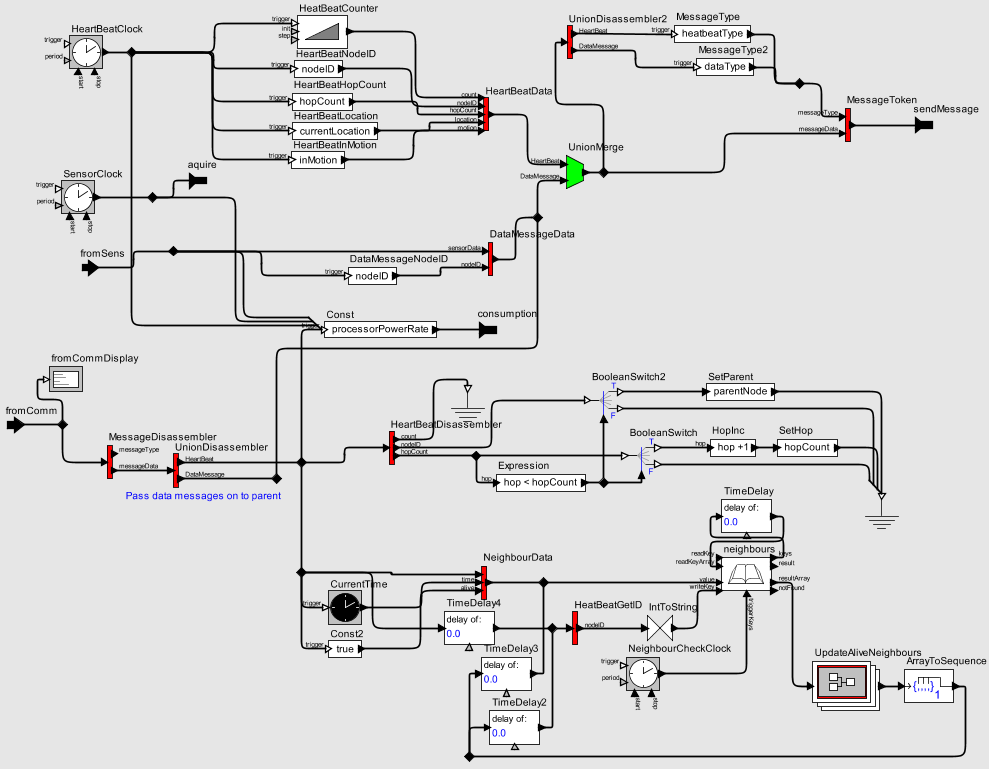
\includegraphics[width=\textwidth]{figures/processorInternals.png}
    \caption{The partially complete actor model of the processor before re-implementation in Java.}
    \label{fig:processorInternals}
\end{figure}

Moving to Java allowed much more complex behaviour to be defined simply and multiple actions / function reuse could take place without the problems of looping connections that introduce the need for `TimeDelay: 0' actors to act as one way connections. The partially complete actor model can be seen in Figure~\ref{fig:processorInternals}.

As the processor controls the behaviour of the nodes it would need to be re-implemented for each algorithm tested. To minimise this the processor class is designed to be extended for each control algorithm, providing all the other necessary components in the base class for re-use. These can always be overridden as needed according to Java's inheritance model.

The processor has three periodic tasks that are controlled by the clocks in the model. Firstly to create heartbeat messages, these are used to communicate the state of nodes throughout the network. The heartbeat is broadcast to all nodes within the communication range --- the neighbours of the node. The node information is used to construct a tree network architecture with the parent node being the one with the shortest hop count to the root node. Secondly to get data from the sensing module and produce application messages to send back to the root. And thirdly to check the state of the known neighbours.

When messages are received from other nodes application data is forwarded on to the parent, eventually reaching the root, and heartbeat messages are stored in a neighbour data store. As the heartbeat period across the network is known the time between heartbeats from neighbours can be used to check if they are still alive --- the reasoning behind the naming of the heartbeat protocol. This time-out is calculated to be larger than the heartbeat period to reduce the likelihood of transient failures. When the neighbour check is carried out the data store of neighbours is update with the alive state for each neighbour. The processor is then able to read this information to trigger recovery.

\subsection{Sensing}

The sensing module is the simplest, it outputs an environment measurement when triggered, this models the behaviour of reading from a sensor board and the power consumption required to do so and gives data to send in the periodic application messages.

\section{Self-Healing Algorithms}

The self-healing algorithms under test are implemented within the processing module. The base Java class for processing can be extended for the specific functionality required by each algorithm.

Wireless network recovery is initiated when a node discovers a neighbouring node is no longer communicating. This could be for a variety of reasons as discussed in Chapter~\ref{cha:LitReview}, how the recovery is dealt with depends upon the particular algorithm used, and it is the algorithms responsibility to recognise the reason for non-communication and react accordingly.

To implement a recovery algorithm the periodically called neighbour check function is overridden.

\subsection{Restoring connectivity through Inward Motion (RIM)}

The RIM algorithm was developed by \citet*{Younis2010}. It was chosen for implementation because of its simplicity and performance, the algorithm is clearly presented and seemingly performs well in low density networks with an even distribution of power consumption. This seemed worthwhile to put to the test, particularly as RIM has become a common comparison algorithm since its development.

Using the pseudocode the algorithm was implemented to run when the neighbour check found a non-communicating node. The algorithm then reacts based upon whether the node seems to have failed or just moved away. Various geometric functions are required to compute the new location depending on how many other nodes are moving.

\begin{algorithm}
\begin{algorithmic}[1]
\If{a sensor node $J$ detects a failure of its neighbour $F$}
    \State{\Call{Notify\_Movement}{$J$}}
    \State{$J$ moves towards $F$ until becoming a distance $r/2$ away}
    \If{$J$ is unable to reach any other 1-hop neighbour of $F$}
        \State{$J$ returns to its original location ($F$ is a boundary node) and sends a do-not-move message to its neighbours.}
    \EndIf
\ElsIf{$J$ receives (a) notification message(s) from $F$}
    \If{$I\_Already\_Reconnected$} \label{rim:noChain}
        \State{Done;}
    \EndIf
    \State{$NewPosition \gets$ \Call{Compute\_newPosition}{$J$}}
    \If{$NewPosition \neq CurrentPosition$}
        \State{\Call{Notify\_Movement}{$J$}}
        \State{$J$ moves to $NewPosition$}
    \EndIf
\ElsIf{$J$ receives a ``do-not-move'' message from $F$}
    \State{$J$ does not move towards $F$ (no cascade movement)}
\EndIf
\State{$I\_Already\_Reconnected \gets TRUE$}

\Function{Compute\_newPosition}{$J$}
\State{$NUM\_PriorNBR \gets$ Number of notification messages that $J$ has received with the lowest rank}
\If{$J$ stays connected with all $PriorNBR$ with least rank}
    \State{\Return{$CurrentPosition$}}
\EndIf
\State{$Location\_Senders[] \gets$ New location(s) of (a) sender(s) from which $J$ have received (a) notification message(s)}
\If{$NUM\_PriorNBR = 1$}
    \State{\Return{a point $r$ unit(s) away from $Location\_Sender[0]$ on the direct path to $Location\_Sender[0]$}}
\Else
    \State{Define a circle of radius $r$ around each of $Location\_Sender[]$}
    \If{$NUM\_PriorNBR = 2$}
        \State{\Return{the closest point between two intersection points}}
    \ElsIf{$NUM\_PriorNBR > 3$}
        \State{\Return{the closest point among intersection points which is located inside all other circles}}
    \EndIf
\EndIf
\EndFunction

\Function{Notify\_Movement}{$J$}
\State{Send a message with a rank value increased by 1 to inform all neighbours of $J$ about its motion and its new position.}
\EndFunction

\end{algorithmic}
\caption{Pseudocode for the RIM algorithm}
\label{alg:RIM}
\end{algorithm}

Upon implementing RIM an interesting edge case was discovered which caused a node (\emph{A}) to move in oscillation until its energy is depleted. This occurs when a node becomes just our of range from two other nodes (\emph{B} and \emph{C}) that have previously moved and set \variable{I\_Already\_Reconnected} true. When the \emph{A} notifies its intention to move \emph{B} and \emph{C} do not respond in chained motion because of lines 8--10 in algorithm~\ref{alg:RIM}, therefore as \emph{A} moves away and loses connection with \emph{B} or \emph{C} it detects them as failed and moves back towards them. When \emph{B} and \emph{C} are either side of \emph{A} this will repeat as one comes into range the other will have become out or range and the cycle continues.

\lstinputlisting[language=Java,firstlineandnumber=60,lastline=89,widthgobble=3,float,caption={Java implementation of RIM},label={lst:RIM}]{../sim/actor/NodeProcessorRIM.java}

The implementation of RIM (algorithm~\ref{alg:RIM}) can be seen in listing~\ref{lst:RIM} which is run periodically for each neighbour of a node.

%\subsection{Simultaneous Failures Recovery Approach (SFRA)}

\section{Simulation Scenarios}

To test the algorithms and the platform a variety of scenarios are constructed for the network to run in. These scenarios, their goals, and the reasoning for their use are presented in this section.

\subsection{Single Node Failure}

The single node failure is a common and simple scenario to perform. Whether due to energy depletion, hardware failure, obstruction to transmission, or a software fault and individual node could fail at any time for many reasons. As seen in the literature, this was the first problem scenario self-healing algorithms were designed to solve, therefore it is the base test as to whether or not they are functional and can be classed as self-healing.

The goal of this scenario is to retain / restore connectivity across the network after a single node has failed. For this scenario the simulation was set up with a number of nodes randomly distributed within a 1000x1000 unit area. Once running a node is randomly selected to fail, where it changes to a non-responsive state no longer sending or receiving messages. RIM is designed with this specific scenario in mind and results are presented with varying communication ranges and numbers of deployed nodes. However when re-creating these experiments it was discovered that the random placement combined with lower range or a lower deployment results in a highly partitioned network: a high number non-connected nodes / clusters than cannot route to the root node.

\begin{table}[]
\centering
\resizebox{\textwidth}{!}{%
\begin{tabular}{|l|l|l|l|}
\hline
Number of deployed nodes & Minimum range deemed suitable & Mean connected nodes & Std. Deviation \\ \hline
25                       & 250                           & 24                   & 1.54           \\ \hline
50                       & 200                           & 47.8                 & 3.34           \\ \hline
100                      & 150                           & 99                   & 1              \\ \hline
200                      & 100                           & 196.8                & 3.4            \\ \hline
\end{tabular}%
}
\caption{Minimum ranges for number of randomly deployed nodes in a 1000x1000 unit area.}
\label{tab:noderange}
\end{table}

The minimum range deemed suitable for this area for the number of deployed nodes is presented in table~\ref{tab:noderange}. As can be seen, these values are much larger parameters than most of the simulations run by \citeauthor*{Younis2010}. It would seem that their random deployments are either non-random enough to create a connected network, or their results for low density networks are incredibly sparse. To test this scenario on my platform the values from table~\ref{tab:noderange} were used as the network parameters.

\subsection{Multi Node Failure}

\subsection{Further Scenarios}

There are several other scenarios that could be developed for the platform. One particularly useful scenario is using an unreliable communication channel. Doing so would produce a more realistic transmission model and show the resilience to real-world problems in communication for the algorithm under test. All kinds of outside actors can affect radio transmission, interference from other sources or even from within the network itself is a major issue in all forms wireless communication. As discussed in the literature, the radio pattern for transmission and reception vary greatly from the ideal fixed radius circle used in the previous scenarios, modelling this degradation would be another challenge, but a worthwhile development to improve the simulation platform.

The wireless channel model in PtolemyII provides power loss modelling and probabilistic transmission loss alongside the limited range properties which have been used. And within VisualSense collision detection is possible by providing a message size / transmission time per transmission. Using these to extend the communications module of the nodes could greatly increase the resemblance to real world environments and allow testing in harsh settings during the development of a self-healing algorithm.

\chapter{Evaluation}
\label{cha:Eval}

Each scenario is run on each of the different sized networks and repeated to produce an average response for that network set-up.

\section{Single Node Failure}

\section{Multi Node Failure}

\chapter{Conclusions}
\label{cha:Conclusion}



\bibliography{project-report}

%author = {\c{C}al\i\c{s}kanelli, \.{I}pek},

\end{document}
